\documentclass{article}
\usepackage[utf8]{inputenc}

\title{Game of Thrones Series Visualization}
\author{Fred Hohman, Sandeep Soni, Ian Stewart\\CS 7450 Project Proposal}
\date{September 14, 2016}

\usepackage{graphicx}
\usepackage[a4paper,%
            left=1.5in,right=1.5in,top=0.5in,bottom=1.0in]{geometry}

\begin{document}

\maketitle

\section*{Problem Addressed}

After watching a TV series, the curious viewer often wants to go back and examine details of the series that were especially interesting or unusual. Unfortunately, high-level summaries of a TV series which can guide the user’s exploration do not exist. We currently lack standardized methods to expose the inner structure of an animated feature, apart from whatever screen-captured images are generated manually by fans after the screening. Visualization that sheds light on the textual and visual qualities of a TV episode can lend insight into the film’s narrative qualities, such as the arc of a storyline or the development of a character. Even better is a system that allows the viewer to compare multiple TV episodes at once, which reveals key similarities and differences across episodes in a series. Fundamentally, our project would treat TV series visualization as a multi-layered time series analysis problem to expose the viewer to high-level attributes of the series. We choose to analyze the HBO series Game of Thrones for its wide cultural appeal, acclaim, and interesting use of both both and dialogue. 

\section*{Data}
\subsection*{Description}
\begin{itemize}
\item \textbf{Images}: We use the visual content of the show by representing the video for each episode as a sampling of still frames at a uniform sampling rate (for example, every one second). A typical episode is around 60 minutes, and there are 60 episodes in total, giving us 216K frames in total.
\item \textbf{Text}: For every episode, we also have the subtitles, providing us with text of the conversations between the characters, but also with useful meta data, like the time of the conversation and the expressions of the characters on the show (e.g \textit{John gets angry}).
\item \textbf{Network}: From the text data, we also plan to induce the social network between the characters on the show, by using different heuristics like a pair of characters are connected if they co-occur within a certain time period. 
\end{itemize}

\subsection*{Analysis}
For our analysis, we plan to extract color attributes from images. By extracting the top colors used each of the frame, we plan to analyze how the color change over the length of an episode, whole season and all seasons. We would also extract sentiment from the text data and visualize it in the same dimensions as the color. By correlating the sentiment with colors, we can get an insight into how scenes with different emotions are created. By using the network connections between the characters we can compare how they are visually and emotionally represented.  

\begin{figure}[h!]
\centering
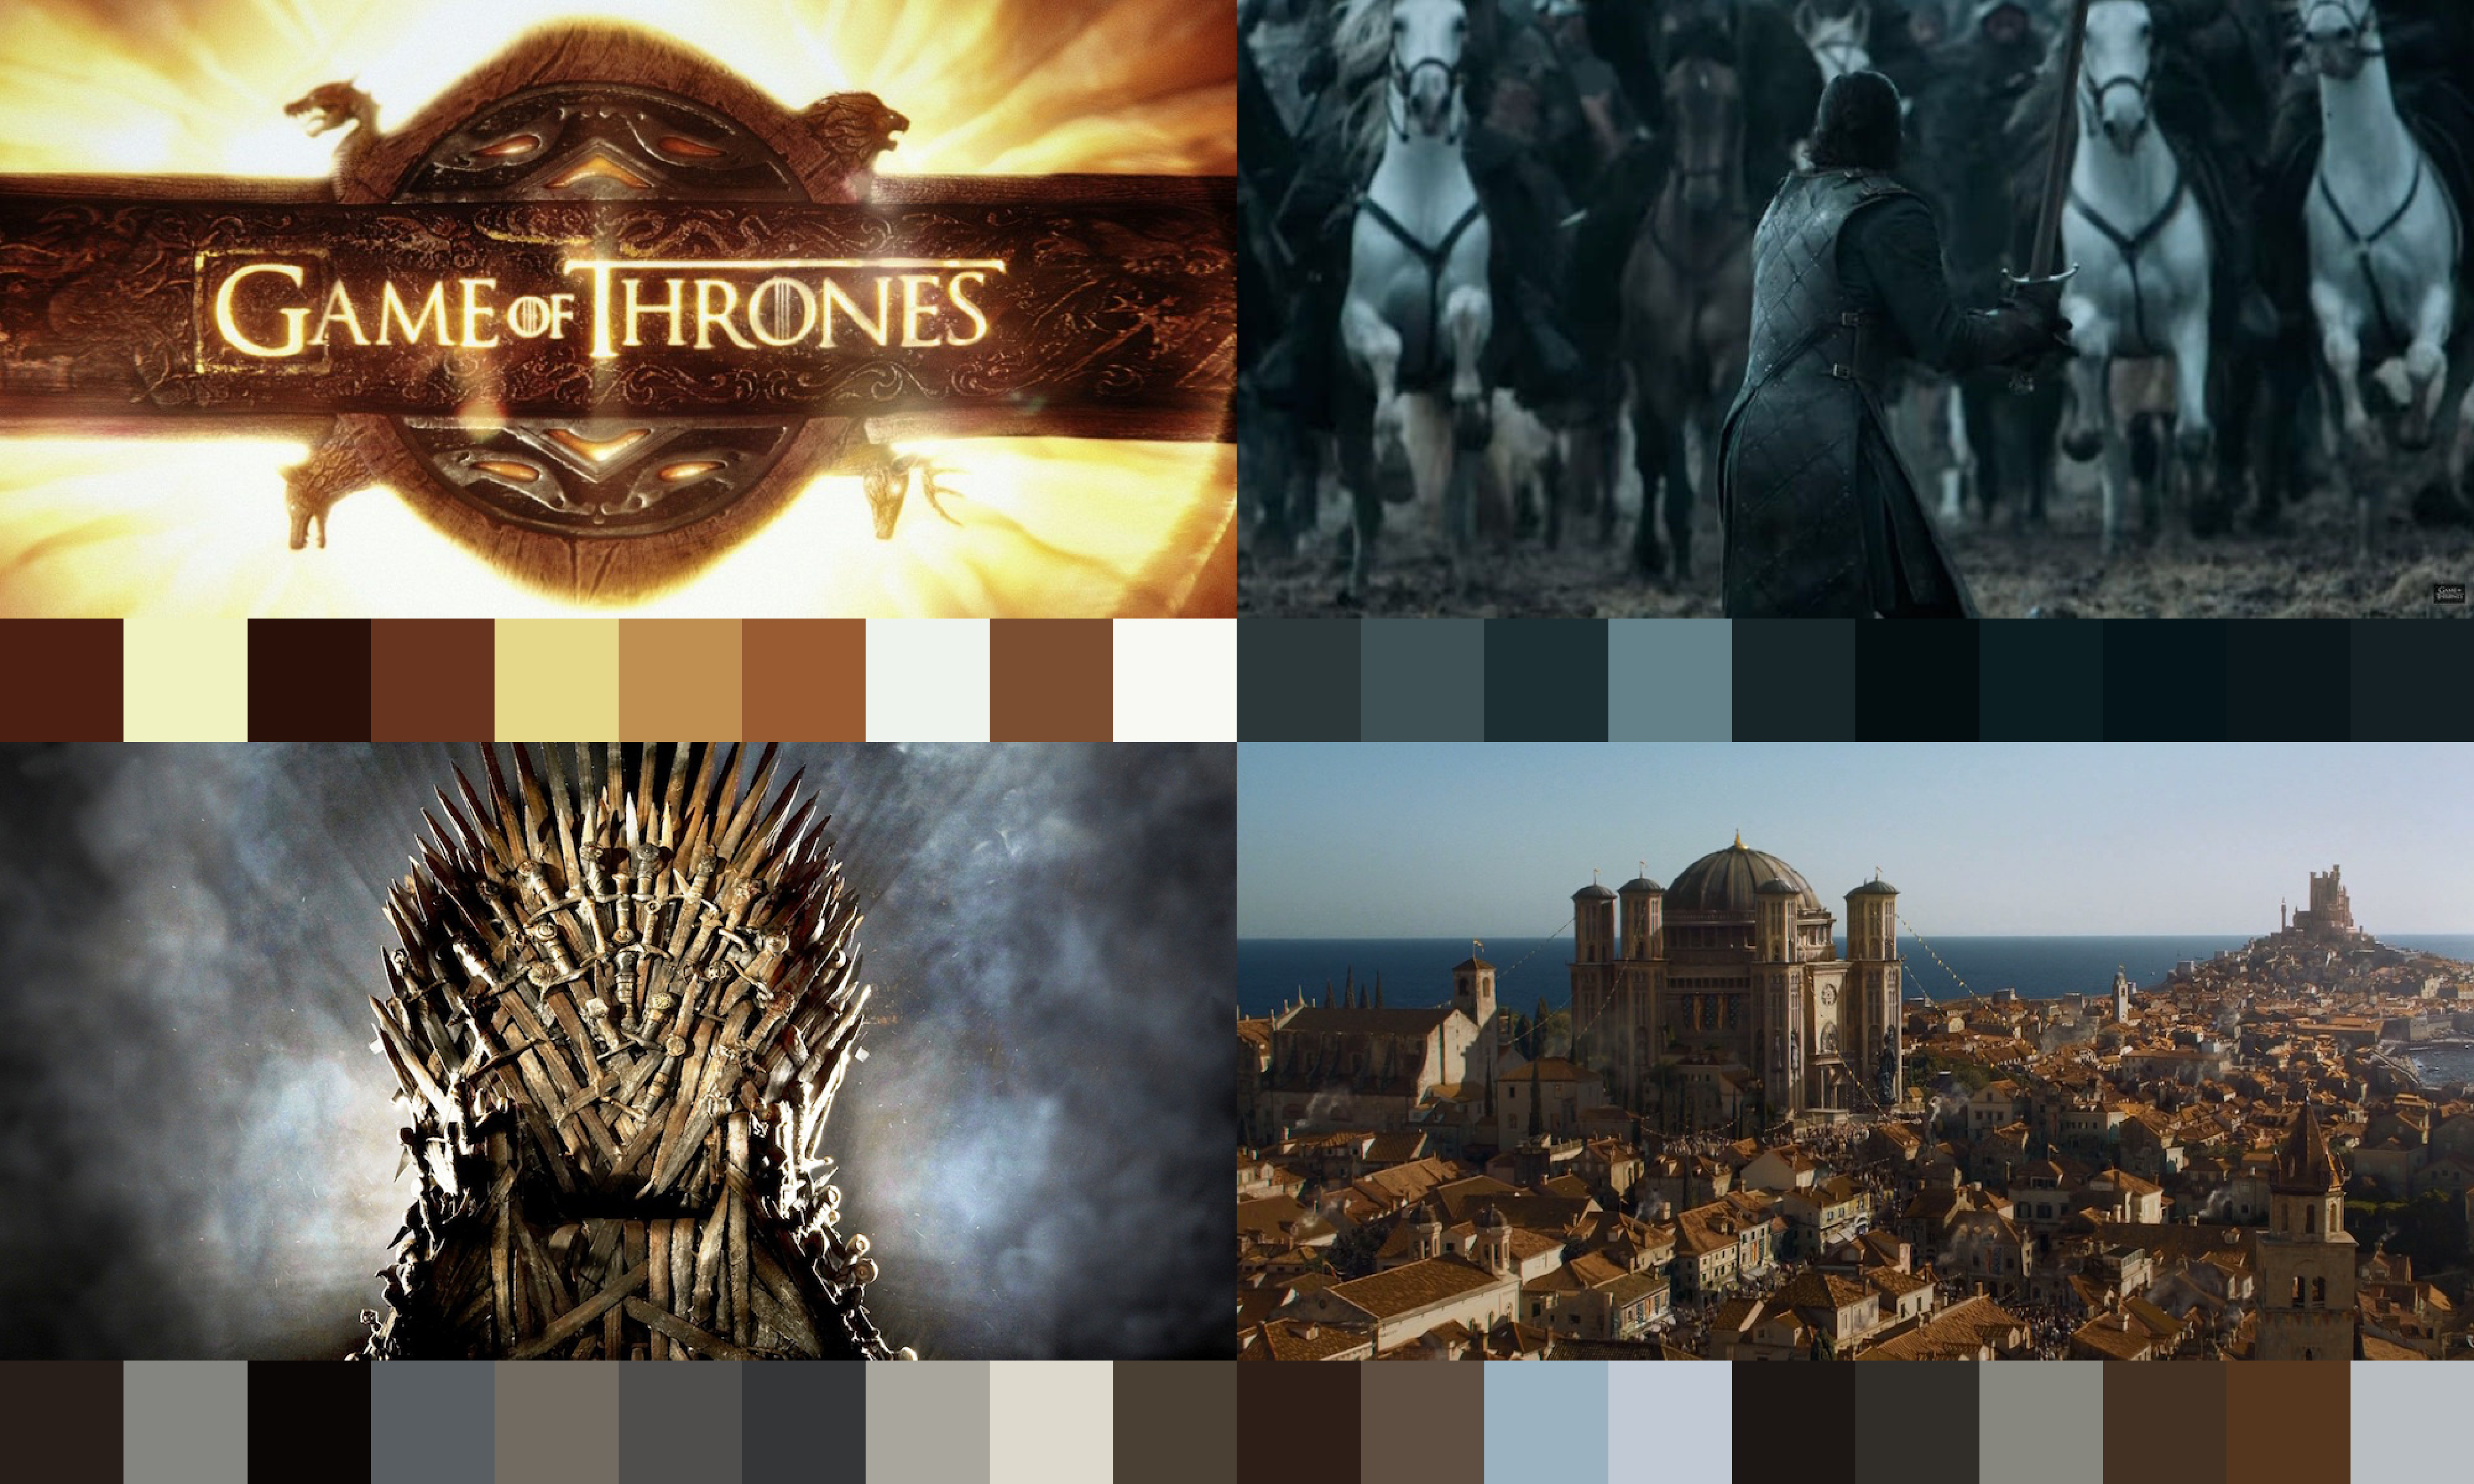
\includegraphics[width=\linewidth]{proposal-fig.pdf}
\caption{Four scenes from Game of Thrones and their associated color palettes. Color palettes are generated from Python code we wrote and can be modified to produce different palettes with different number of colors.}
\label{fig:proposal-fig}
\end{figure}

\section*{Target Audience}

The visualization would serve any fan or critic of a series who wants to uncover how a particular part of the show fit into the overarching plot. This is especially applicable since we will make the system interactive, such that fans can zoom in and out of regions of interest (e.g. within a season or across multiple seasons) to make ``deep dives'' in addition to the ``big picture'' view. The visualization will provide evidence to a fan who wants to make a particular argument about the TV series, such as how a certain season is disliked by fans because of its consistently dull colors. In addition to current fans, the  visualization could help future fans decide whether or not to watch the series based on the representative colors or text sentiment.

Conversely, the visualization could also help the TV show's directors and artists to better understand the big picture behind their day-to-day plans. A new set designer on Season 2 of Game of Thrones, for instance, could use the visualization to get a better understanding of the color scheme of the previous season.

\section*{Potential Questions}

We list several questions for analysts to explore:

\begin{enumerate}
    \item How does color change across the series? A fan would like to see whether a particular season was characterized by a specific set of colors and how that matched the overall mood of the season. 
    \item Do changes in sentiment correspond to changes in the color palette? For instance, if most of the images are dark grays but one scene is in full color, we may see a corresponding spike in positive sentiment.
    \item How do the words and colors associated with characters change over time? If a user queries a certain character, e.g. Cersei Lannister, who is known to occupy a fixed role across the series, we might expect the scenes associated with that character to have a consistent color palette.
    \item Which season of the show was the most surprising in terms of its visual and textual trajectory? Pinpointing unexpected combinations of color and sentiment could help fans understand what made a particular season especially exciting or controversial.
\end{enumerate}

\end{document}
